\documentclass[sigconf]{acmart}

\usepackage{url}
\usepackage{hyperref}
\usepackage{lipsum}
\usepackage{graphicx}

\graphicspath{{images/}}

\renewcommand\footnotetextcopyrightpermission[1]{} % removes footnote with conference information in first column

\title{Analyzing Temporal Trends and User Modeling\\ on an Online Chess Community}
\subtitle{IN4252 - Web Science and Engineering}
\author{Santhos Baala Ramalingam Santhanakrishnan}
\affiliation{TU Delft - Student Number 4740270}
\email{S.B.RamalingamSanthanakrishnan@student.tudelft.nl}

\begin{abstract}
Lichess is a crowdfunded online chess community with over 250 million recorded games since 2013. In this draft paper, we explore the public game dataset for general and temporal trends, corresponding to player levels, identify choices of top chess players over feasible time periods and answer questions that arise along the way. We also compare the online trends against the real-world ELO distribution to gain insights on specifics of the Glicko rating system, compared to the real world FIDE ELO and its effect on user retention. Using the insights we try to draft the features of an online chess player, that acts as a basis for further user modeling and merging with profiles from other social networks. From a domain point of view, we identify user preferences such as opening choices, preferred time control, frequency of visits to gauge overall involvement in the community.
\end{abstract}

\setcopyright{none}
\settopmatter{printacmref=false}
\acmPrice{}
\acmISBN{}
\acmDOI{}

\begin{document}

\acmConference[IN4252]{Web Science and Engineering - Final Paper}{Jan 15 2017}{EEMCS, TU Delft}

\maketitle

\section{Introduction}

Lichess \footnote{\url{http://lichess.org}} is a free online chess community, started in 2013 and it peaked in 2017 with over a million games played every single day across various time controls and chess variants. It is crowd-funded, open source and each game is recorded, resulting in a large public dataset with rich meta data and domain-specific chess information. Chess is a cognitive-heavy game and has been time and again a sample space for understanding human psychology and the vastness in available data has been a paradise for statisticians to elicit interesting patterns, the extent to which, display of skills in chess has been correlated to excellence in academics and other cognitive abilities.

Insights gained from analyzing Lichess shall help form a basis for future work on how to model and incentivise a wide range of  online learning processes in order to create strong retention, where the cognitive abilities are being challenged. Also, skill building on Lichess itself is a non-trivial and a long term problem and we need more insights on providing a tangible improvement path for users, more in the line of MOOCs \footnote{Lichess TV: \url{https://lichess.org/tv}, Lichess Learn: \url{https://lichess.org/learn}}, and recommend courses based on observed skill and behaviour.

\textbf{TODO: A paragraph on the structure of the rest of the paper.}
\lipsum[1]

\section{Related Work and Dataset}

Analysis from a cognitive science standpoint has been carried out on chess databases by \cite{vaci2017chess}, in which the authors have taken up the German national chess database and laid out methods to carry out analysis on skill development over lifetime, birth cohort effects, effects of activity and inactivity, etc. Contrary
to the analysis in \cite{vaci2017chess}, we do not have any skill or recording restrictions in Lichess, however lack
of demographic information in the available dataset restricts the kind of analysis that we can perform. 

A common feature of competitive sports is measuring the relative skill of a player, usually quantified as ELO points through a rating system (compared by \cite{vevcek2014comparison}), of which the Glicko-2 \cite{glickman1995glicko} rating system is adopted by Lichess. An important difference to be noted in our dataset is that ratings of a player 
are calculated and assigned in real-time (at the end of each game) whereas in the real world rating lists are
published periodically, typically monthly or quarterly, which means a recorded game could actually be reflecting a
shadow rating. This leads to high volatility of the Glicko's $RD$ factor in Lichess. For feasibility reasons, we
analyze only a subset of the available data \footnote{\url{http://database.lichess.org}}, between 2013-Jan-1 and 2014-Jan-31 in three game formats -- bullet, blitz, classical and correspondence. The dataset, after cleanup of data, contained a total of 4,071,927 games, consisting of bullet - 1,086,961 (26.694\%), blitz - 1,576,431 (38.715\%), classical - 1,399,978 (34.381\%) and correspondence - 8,557 (0.21\%) games respectively. A total of 54,058 unique players and their corresponding profiles were captured from the dataset. The list of features of a game and a player are given in detail along with an example in appendix.

\section{Analysis}

We first start with basic temporal observations to develop an understanding of the dataset and then move on to features that we consider for user modeling. \autoref{fig:games_played} shows the timeline of games played in various formats, we observe that there are spikes and valleys, which were found to be strongly correlating to new users (coefficient of 0.87) joining daily \footnote{One caveat is that, day refers to an UTC day throughout the paper.}, no relation was found between days of week though.

\begin{figure}[htbp]
\caption{Games played over time by type}
\label{fig:games_played}
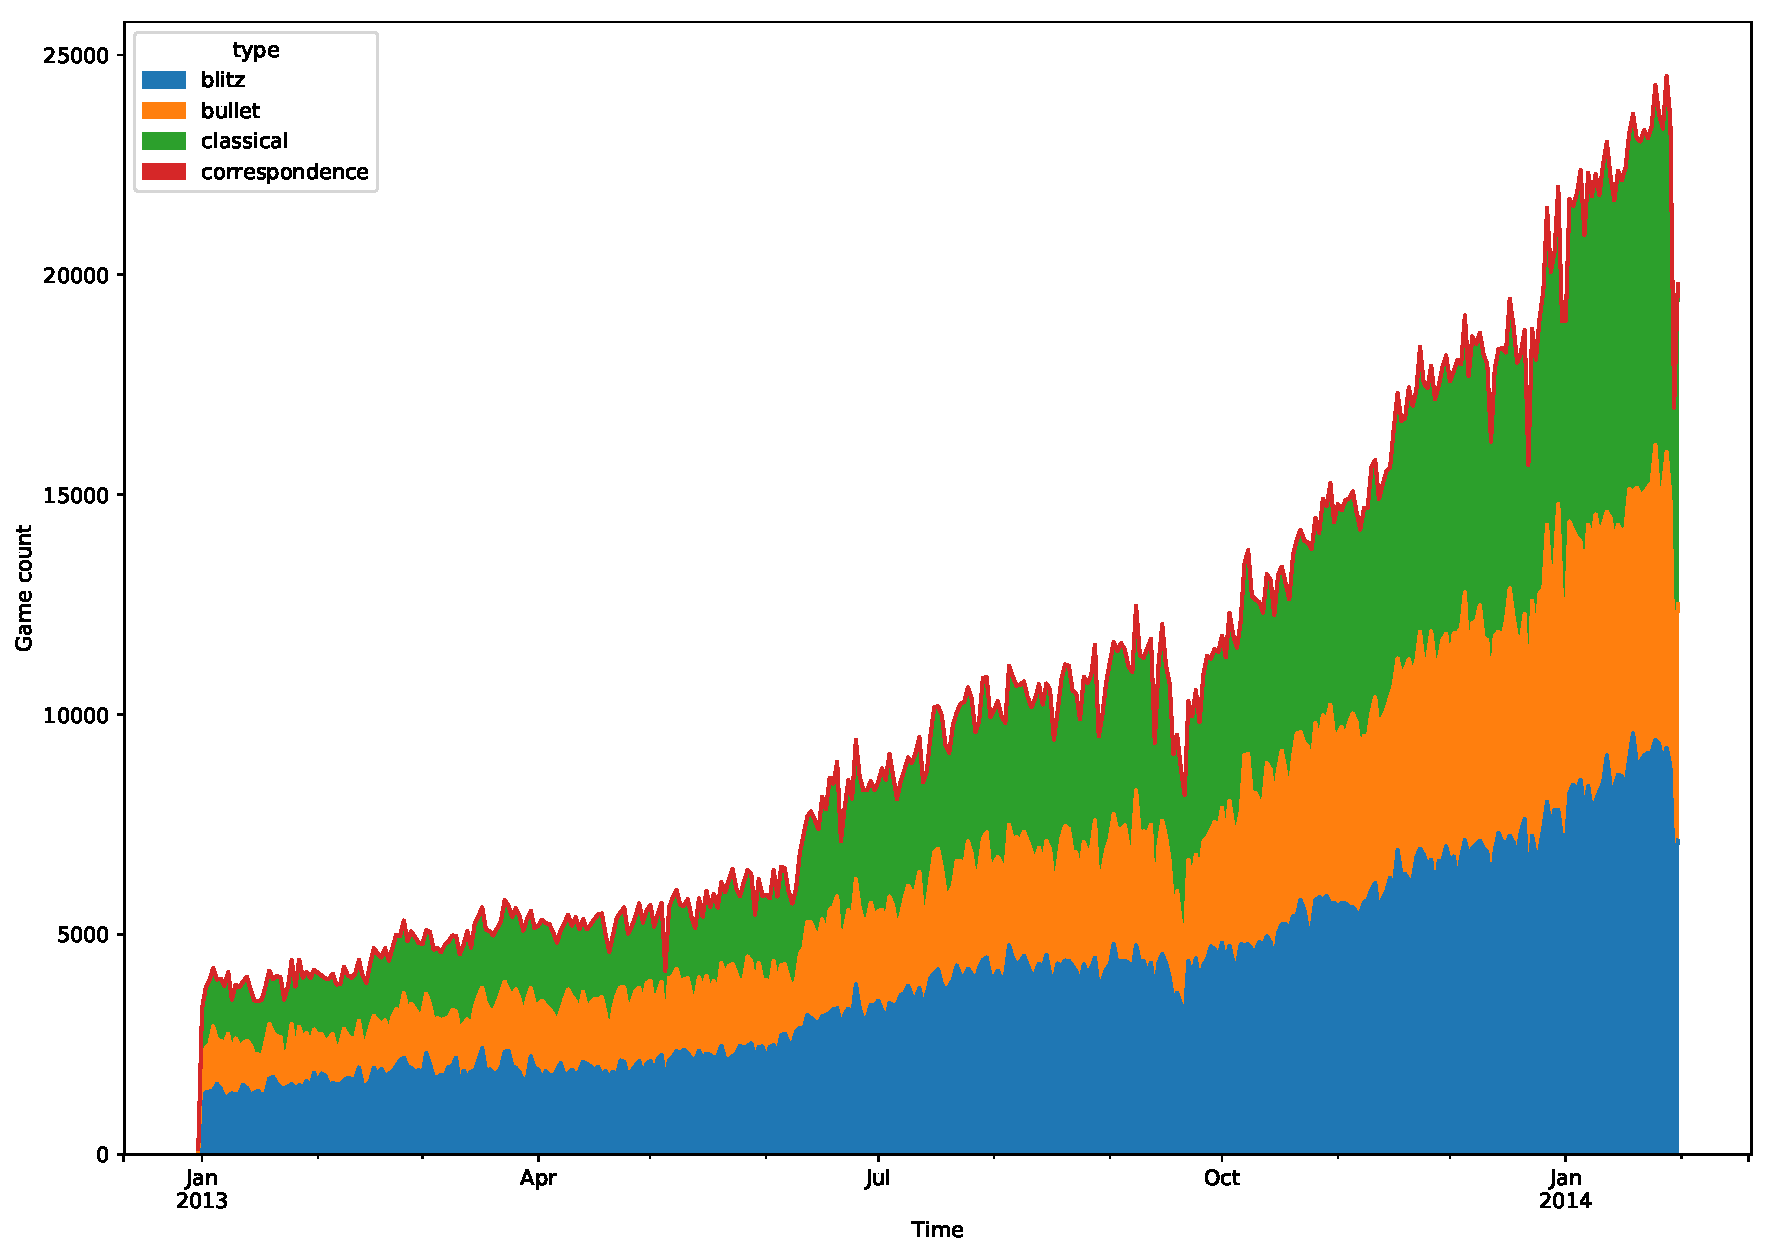
\includegraphics[width=0.5\textwidth]{games_played}
\end{figure}

\autoref{fig:rating_probability_density} shows the probability density function of player ratings (elo) in the system,
by min, max and mean ratings. We clearly see that there is huge spike at $1500$ and sub-peaks at around 700 points above and below 1500. This is contrary to the analysis in \cite{vaci2017chess} and FIDE elo ratings in general. This is due to the fact that real-world rating systems never assign a rating to a new player unlike Lichess, which assigns 1500, based on the Glicko-2 documentation \cite{glickman1995glicko}. A close correlation was found between elo points  and the $RD$ factor (-0.007658) and due to skew from a large number of data points at 1500, it was slightly negative stabilizing as it approached higher elos, visible through descriptive statistics in \autoref{table:elo_descriptive_stats}. The max and min $RD$ explains the sub-peaks in \autoref{fig:rating_probability_density}. This leads us to the question \textit{Are weaker players majority contributors to the Lichess database?}.

\begin{figure}[htbp]
\caption{Rating distribution in blitz games}
\label{fig:rating_probability_density}
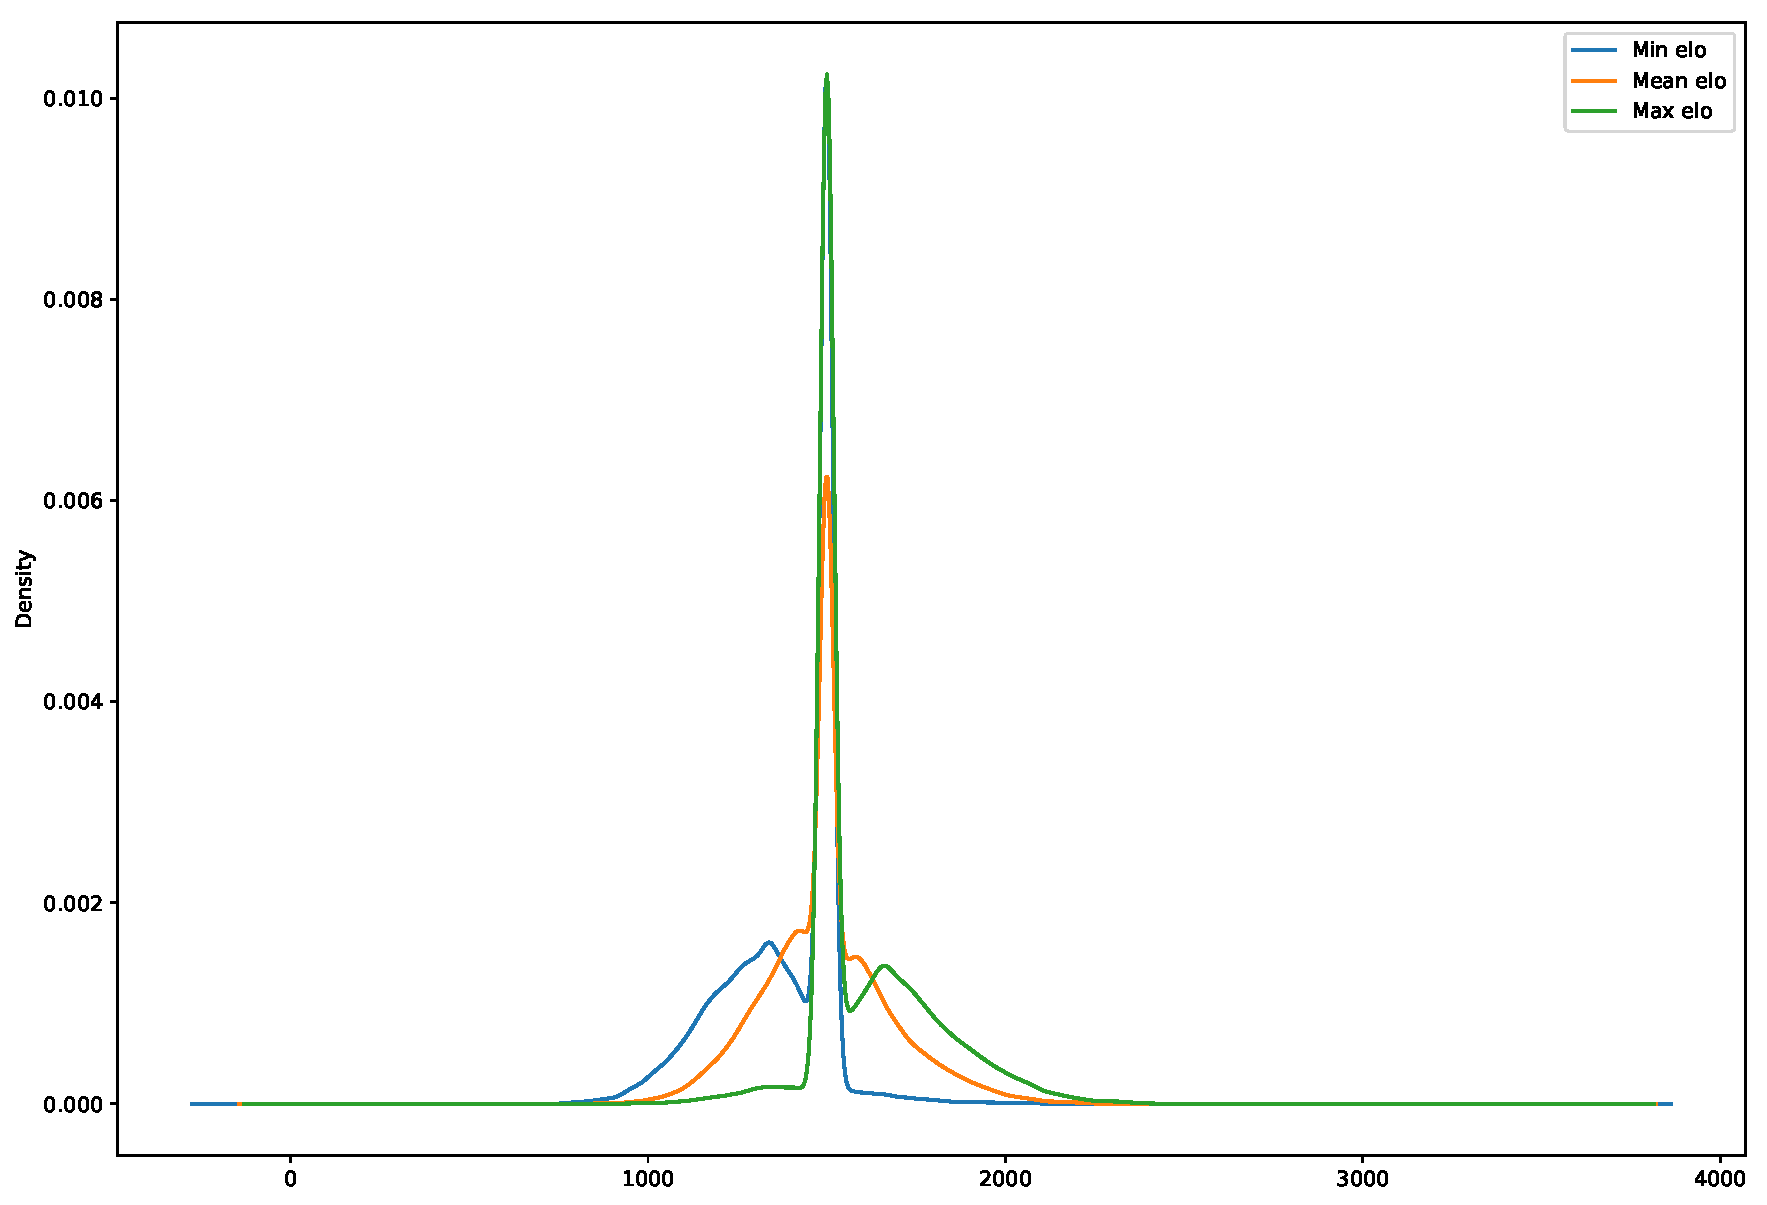
\includegraphics[width=0.5\textwidth]{blitz_rating_distribution}
\end{figure}

\begin{table}[htbp]
\caption{Elo and $RD$ factor descriptive statistics}
\label{table:elo_descriptive_stats}
\begin{tabular}{|c|c|c|}
  \hline
  Stat & Elo & RD \\
  \hline
  mean & 1605.25 & -0.671 \\
  std & 214.83 & 34.64 \\
  min & 0 & -624.000 \\
  25\% & 1467.00 & -10.00 \\
  50\% & 1607.00 & 0.00 \\
  75\% & 1751.00 & 10.00 \\
  max & 2828.00 & 649.00 \\
  \hline
\end{tabular}
\end{table}

\section{Discussion}

\section{Conclusion}

\bibliographystyle{abbrv}
\bibliography{wse-final-paper}

\section*{Appendix}
\begin{appendix}

\end{appendix}

\end{document} 

